\documentclass[12pt]{article}

%margó méretek
\usepackage[a4paper,
inner = 35mm,
outer = 25mm,
top = 25mm,
bottom = 25mm]{geometry}


%packagek, ha használni akarunk valamit menet közben
\usepackage{lmodern}
\usepackage[magyar]{babel}
\usepackage[utf8]{inputenc}
\usepackage[T1]{fontenc}
\usepackage[hidelinks]{hyperref}
\usepackage{graphicx}
\usepackage{amssymb}
\usepackage{epstopdf}
\usepackage{setspace}
\usepackage[nottoc,numbib]{tocbibind}
\usepackage{setspace}
\usepackage{wrapfig}
\usepackage{float}
\usepackage{blindtext}
\usepackage{enumitem}

\setstretch{1.5}
\begin{document}
	
	

\begin{titlepage}
	\vspace*{0cm}
	\centering
	\begin{tabular}{cp{1cm}c}
		\begin{minipage}{4cm}
			\vspace{0pt}
			
\includegraphics[width=1\textwidth]{elte_cimer}
		\end{minipage} & &
		\begin{minipage}{7cm}
			\vspace{0pt}Eötvös Loránd Tudományegyetem \vspace{10pt} \newline
			Informatikai Kar \vspace{10pt} \newline
			Komputeralgebra Tanszék
		\end{minipage}
	\end{tabular}
	
	\vspace*{0.2cm}
	\rule{\textwidth}{1pt}
	
	\vspace*{4cm}
	{\Huge Gépi tanulás a legynagyobb sebzés eléréséhez }
	
	\vspace*{9cm}
	
	\begin{tabular}{cp{1cm}c}
		\begin{minipage}{7cm}
			\vspace{0pt}Dr. Vatai Emil \vspace{10pt} \newline
			Adjunktus \newline
			Komputeralgebra tanszék \newline
			ELTE IK
		\end{minipage} & &
		\begin{minipage}{7cm}
			\vspace{0pt}Szalóki Sándor \vspace{10pt} \newline
			Programtervező informatikus BSc.
		\end{minipage}
	\end{tabular}
		
	
	\vfill
	
	\vspace*{1cm}
	Budapest, 2018
\end{titlepage}

\tableofcontents
\newpage

\section{Bevezető}

Legfőbb célom a szakdolgozattal a gépi tanulás mélyebb megértése, tanulása egy olyan példán keresztül, amely előfordulhat problémaként a való életben is.
\newline
A probléma, amivel itt foglalkozunk kellően bonyolult ahhoz, hogy a megoldásához gépi tanulást kelljen alkalmazni és megoldása ne legyen triviális egy egyszerű algoritmussal.
\newline
Ahhoz, hogy a feladat több legyen, mint egy egyszerű út keresés, minden lépés hatással van a környezetére, illetve a környezettől függően egy-egy lépés hatása, értéke változhat.
\newline
Erre egy kellő nehézségű probléma a Final Fantasy XIV harcrendszerének szimulálása, majd ebben a szimulációban való tanulás.

\pagebreak

\section{Felhasználói dokumentáció}

\subsection{Feladat}

\subsubsection{Játék modell}

Első feladat a játéknak egy kellő pontosságú modellezése. A megoldás hatékonysága érdekében törekedni kell arra, hogy ne legyen felesleges adat, viszont minden, ami szükséges, az elérhető legyen. 
A harcrendszer szabályai pontosan meghatározhatóak, így a szimulációtól elvárható a pontos eredmény is. 
Két fő részre osztható a modell: Karakterek és ezek képességei.

\paragraph{Karakterek}

Minden karakternek három meghatározó eleme van:

\begin{description}[align=right,labelwidth=3cm]
	\item [Gyorsaság] Ez adja meg a karakter globális időzítőjét
	\item [Támadás] A képesség, ami a játékos irányítása nélkül történik a karakter gyorsaságától függően
	\item [MP/TP] Magic Points, illetve Tactial Points, ezek a képességek erőforrásai
\end{description}

\paragraph{Képességek}

Egy képesség leírásához hét tulajdonság szükséges:

\begin{description}[align=right,labelwidth=3cm]
	\item [Potenciál] A sebzés mértékének alapja
	\item [Időzítő] Meghatározza, hogy az adott képesség a globális időzítőt, vagy a sajátját használja
	\item [Erőforrás] A használatának ára MP, vagy TP-ben
	\item [Combo] Képességek adott sorrendben használata esetén más-más lehet egy képesség hatása
	\item [Típus] Fegyver, vagy varázslat
	\item [Feltétel] A használatára vonatkozó feltétel
	\item [Hatás] Használat után adott ideig hatással lehet a következő képességere, a hős állapotára, vagy adott időközönként plusz sebzést okozhat
\end{description}

A karakter tulajdonságai és képességeinek listája alapján egy adott képesség sorozatból készíthető egy szimuláció, amely megadja, hogy a sorozatot hány tizedmásodperc végrehajtani, illetve végrehajtás után ennek mekkora a teljes sebzési értéke.
\newline
Fontos, hogy a szimuláció bármely pontján tudjuk, hogy mi a játékos pontos állapota: Erőforrásainak, globális időzítőjének, képességeinak saját időzítőjének állapota, az aktív hatások, illetve ha van, akkor a Combo álltal meghatározott következő képesség.
\newline
Ez az állapot megfelel annak, amit a játékos játék közben a képernyőn láthatna.

\subsubsection{Gépi tanulás}

A feladat ebben a szimulációban egy olyan képesség sorozat keresése, amely eléri a felhasználó álltal megadott időt, és ezalatt az idő alatt minél hatékonyabb legyen, azaz a legnagyobb sebzés elérésére törekszik.
\newline
A probléma tér elég nagy ahhoz, hogy egy egyszerű kereső algoritmus futási ideje túl nagy legyen. Ennek megoldásához megerősítéses tanulást használ a program.
\newline
Ehhez szükséges, hogy a játék állapotáról egy kellően pontos képet kapjunk, erre szolgál a játék szimulációjából tudható képszerű adat. Ezt az adatot állapotnak, a képességeket pedig akcióknak használhatjuk fel.

\subsubsection{Grafikus felület}

Szükséges egy egyszerű grafikus felület, amely megkönnyíti a program használatát, átláthatóságát. A képességek sorozatának egy megjelenítését, a gépi tanulás eredményének grafikus feldolgozását.
\newline
Az algoritmus eredményessége jól bemutatható néhány egyszerű grafikonon.

\pagebreak

\subsection{Módszerek}

A feladat megoldása funkcionális programozással történik.

\subsubsection{Játék model}

Az említett két fő elemet (Karakterek és Képességek) megfelelő típusokkal felvesszük, majd egy-egy tetszőleges karaktert a képességeivel együtt már egyszerűen előállíthatunk.
Miután kellő adat birtokában vagyunk, a képességekből összeállíthatunk egy sorozatot, amit szimulálni szeretnénk.
\newline
A játék harcrendszerének szimulációja három lépésben történik.
\begin{enumerate}
	\item A képességek sorozatát validálni kell. Ellenőrizni kell, hogy a képesség időzítője szerint lehetséges-e már a használata, rendelkezésre áll-e megfelelő típusú és mennyiségú erőforrás. Illetve néhány képesség rendelkezhet saját feltétellel, amit szintén ellenőrizni kell. Amennyiben minden rendelkezésre áll, a képességet meg kell tartani és a megfelelő hatásokat, illetve időzítőket be kell állítani.
	\item A validált sorozaton végig kell menni és minden ponton az adott állapot szerint ki kell számolni, hogy abban a tizedmásodpercen mennyi sebzés történt, majd ezeket összegezni.
\end{enumerate}

\subsubsection{Gépi tanulás}

A megfelelő algoritmus választásához több tényezőt is figyelembe kell venni. A játék harcrendszerének teljes működése kellően bonyolult, így a működést kihasználó algoritmusok használata bonyolult, ha lehetséges. 
Az akciók értéke az állapottól függ, illetve az akciók változtathatják az állapotot, emiatt az a feladat nem vezethető vissza egy egyszerű többkarú rabló problémára sem.
\newline
A probléma megoldásához Monte-Carlo-módszer használható. Az algoritmusnak nincs szüksége a háttérben működő szimuláció pontos leírására, elég ha tudunk adni egy pontos képet az állapotról, illetve az adott állapotban választott akciók értékéről.
\newline
A szimulációt olyan módon működik, hogy megfelelő képet tudjon adni az állapotról, az akció értéke pedig megadható az képesség sebzésének függvényében.

\subsubsection{Grafikus felület}

A program nem igényel bonyolult grafikus felületet. Egyszerű MVVM architektúra használatával épül fel WPF segítségével. 
Karaketerenként a kilistázzuk a képességek képeit, amelyek majd választhatóak lesznek szimulációra. Lehetőséget kell adni az eredmény sorozatnak kilistázására, illetve grafikonok rajzolására.
Fontos, hogy a számolás a háttérben fusson, hiszen ez egy idő után nagy számításokkal járhat, ami zárolhatja az ablakot.

\subsection{Rendszer-követelmények, telepítés}

A program futtatásához Windows operációs rendszer szükséges. Telepítés nem szükséges, viszont a futtatható állomány mellé el kell helyezni a (programmal együtt kiadott) dinamikus könyvtárakat is.

\paragraph{Ajánlott hardware:} 

Quad-Core 2.3 Ghz processzor, 2 GB RAM

\paragraph{Software követelmény:} 

Microsoft .NET Framework 4.6.1

\pagebreak

\subsection{A program használata}

A program indításához a futtatható állomány szükséges. Ennek indításával rögtön egy ablak fogad (\ref{fig:start}). Az ablakon található egy menüsor rendre Add, Start, illetve Cancel gombokkal. Alatta található a program futásához szükséges beállítások mezői. Egy listában találhatóak a karakterek és hozzájuk rendelt képességek listája. Az ablak közepén kerül majd megjelenítésre a tanult képesség sorozat, majd alatta a két grafikon. Továbbá található még egy státusz sor a képernyő legalján. Ebben a következő információk találhatóak: 

\begin{description}[align=right,labelwidth=3cm]
	\item [Status] Rövid üzenet a program állapotáról
	\item [Generations] A jelenlegi generáció száma
	\item [Damage] A tanult képesség sorozat álltal elért sebzés értéke
	\item [Duration] A tanult képesség sorozat álltal elért idő tizedmásodpercben
	\item [Bar] Töltő csík, amely mutatja, ha éppen számolás történik a háttérben
\end{description}

\begin{figure}[H]
	\begin{center}
		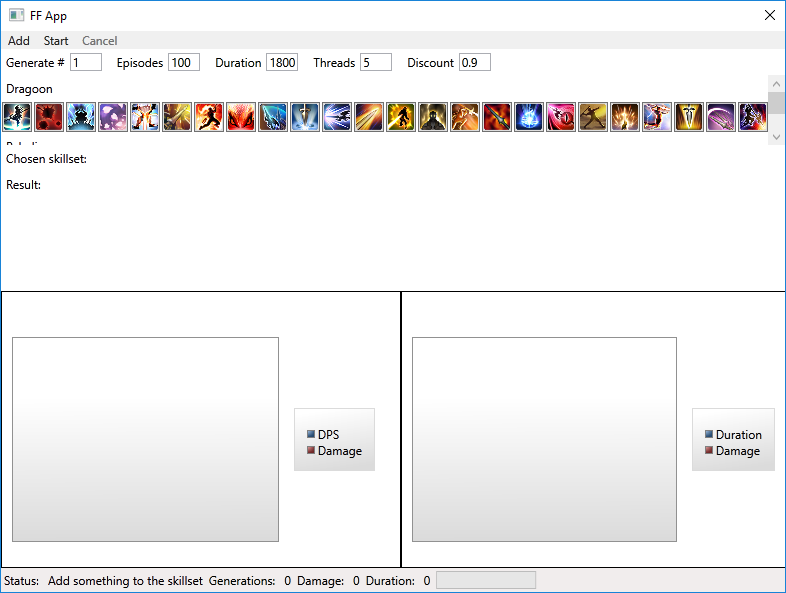
\includegraphics[width=1\textwidth]{start}
	\end{center}
	\caption{Kezdő képernyő}
	\label{fig:start}
\end{figure}

Mielőtt elindíthatnánk a tanulást, választanunk kell egyet a megadott karakterek képességlistái közül (\ref{fig:skilllist}). Minden képesség lista fölött megtalálható a hozzá tartozó karakter neve. A kurzor egy képességen tartása után megjelenik a képesség neve, rövid leírása. 

\begin{figure}[H]
	\begin{center}
		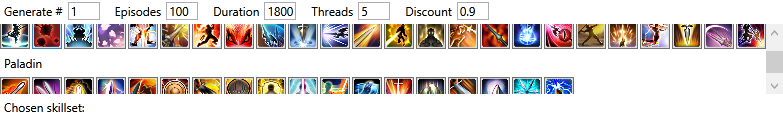
\includegraphics[width=1\textwidth]{skilllist}
	\end{center}
	\caption{Lehetséges választható listák}
	\label{fig:skilllist}
\end{figure}

Ha megtaláltuk a megfelelő listát, akkor az Add menüpontban (\ref{fig:addmenu}) választhatjuk ki a szükséges listát név alapján. Fontos, hogy ilyenkor még szabadon cserélhetjük a karaktert, ez a menüpont Start-ra kattintás után nem lesz előrhető. (Kivéve a New gomb)

\begin{figure}[H]
	\begin{center}
		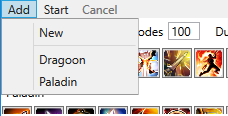
\includegraphics[width=0.4\textwidth]{addmenu}
	\end{center}
	\caption{Lehetséges választható listák az Add menüpont alatt}
	\label{fig:addmenu}
\end{figure}

A lista kiválasztása után erről információt kapunk, a választott lista megjelenik a Chosen skillset alatt (\ref{fig:chosen}). Ezen a ponton a tanulás elindítható a Start gombbal.

\begin{figure}[H]
	\begin{center}
		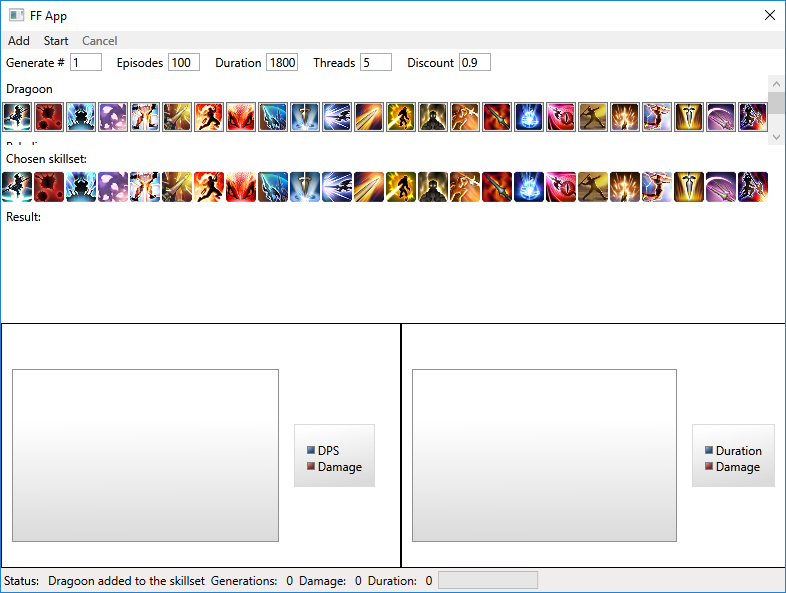
\includegraphics[width=1\textwidth]{chosen}
	\end{center}
	\caption{A választott lista megjelenik a képernyőn}
	\label{fig:chosen}
\end{figure}

Indítás előtt lehetőségünk van néhány beállítás változtatására (\ref{fig:options}).

\begin{figure}[H]
	\begin{center}
		
\includegraphics[width=0.7\textwidth]{options}
	\end{center}
	\caption{Futási beállítások}
	\label{fig:options}
\end{figure}

A beállítások sorra:

\begin{description}[align=right,labelwidth=3cm]
	 \item [Generate] A kívánt generációk számát adhatjuk meg
	 \item [Episodes] Generációnként létrehozott szimulációk száma
	 \item [Duration] Szimulációk hossza tizedmásodpercben
	 \item [Threads] Párhuzamosítás során használható magok száma
\end{description}

Amennyiben a beállításokat megfelelőnek találjuk, a Start gomb (\ref{fig:startgen}) lenyomásával elindítható a beállított számú generációk generálása. 

\begin{figure}[H]
	\begin{center}
		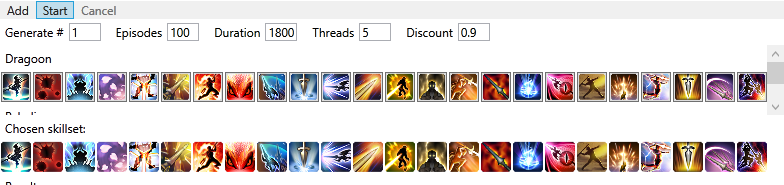
\includegraphics[width=1\textwidth]{startgen}
	\end{center}
	\caption{Generálások indítása}
	\label{fig:startgen}
\end{figure}

A program a generációkat egyesével állítja elő és rajzolja őket ki a képre (\ref{fig:15gen}). Eközben a beállítási mezők, illetve az Add és Start gombok nem elérhetőek, viszont a generálás bármikor leállítható a Cancel gombra kattintva.
Leállítást kérése esetén az éppen futó számolás még befejeződik, ennek eredménye megjelenik a képernyőn, majd az eddig letiltott mezők, gombok feloldásra kerülnek.

\begin{figure}[H]
	\begin{center}
		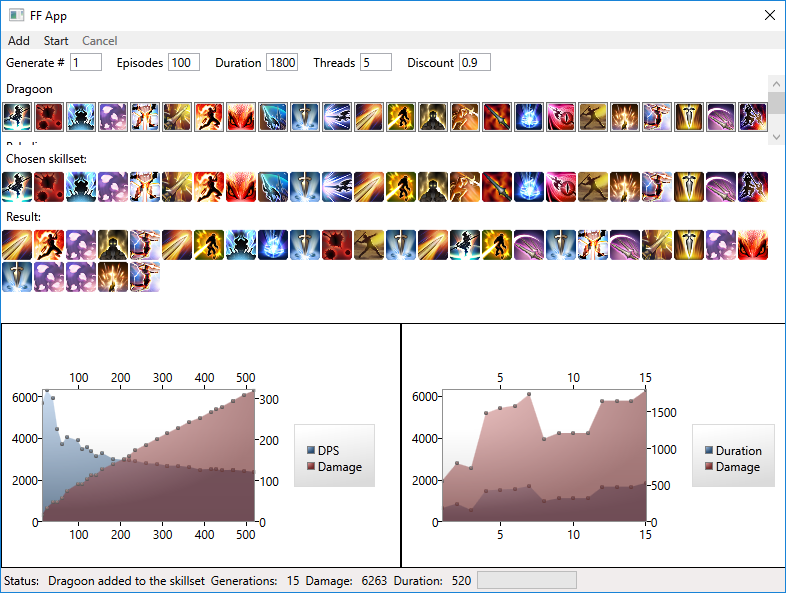
\includegraphics[width=1\textwidth]{15gen}
	\end{center}
	\caption{Eredmény 15 generáció futtatása után}
	\label{fig:15gen}
\end{figure}

Az eredményről három féle információt kapunk. 

\begin{description}[align=left,labelwidth=3cm]
	\item [Result] A jelenlegi tudás alapján generált képesség sorozat
	\item [Bal grafikon] A Result-ban szereplő képesség sorozat szimulálása során kapott sebzés értékek másodpercre osztott értékei. Kék színnel és Damage névvel jelölt terület mutatja az adott másodpercben elért teljes sebzést. Piros színnel és DPS névvel jelölt terület mutatja az adott másodpercben elért sebzés és idő hányadosát.
	\item [Jobb grafikon] Nyomon követhetjük minden generáció tudásának sebzés értékét
\end{description}

Amennyiben újra szeretnénk kezdeni a tanulás folyamatát, az Add menüpont alatt (\ref{fig:addmenu}) található egy New gomb, amivel alaphelyzetre állíthatjuk a programot. Ilyenkor a kiválasztott képesség lista nem változik, ennek változtatásához a programot újra kell indítani.

\section{Fejlesztői dokumentáció}

\subsection{Specifikáció}

\subsection{Módszerek}

\subsubsection{Fogalomtár}

\subsubsection{Játék model}

\subsubsection{Gépi tanulás}

\subsubsection{Grafikus felület}

\subsection{Szerkezet}

\subsubsection{Külső függőségek}

\subsubsection{Adatszerkezetek}

\subsubsection{Modulok}

\subsubsection{Képességek}

\subsection{Tesztelés}

\end{document}